\begin{frame}[fragile]{Mayer Vietoris}
\begin{figure}
\begin{tikzpicture}[scale=.5, y=0.6pt, x=.75pt]
     %row 1
%     \node[font=\large] at (-50, 800) {$(K, U)$};
     \draw[fill=afragreen, draw = black,  line width=2]  (47,800) circle (10pt);  
     \draw[fill=afragreen, draw = black, line width=2]  (117,800) circle (10pt);   
     \draw[fill=afragreen, draw = black, line width=2]  (190,800) circle (10pt); 
     \draw[fill=afragreen, draw = black, line width=2]  (261,800) circle (10pt); 
     \begin{pgfonlayer}{edges}
            \path[draw=black,fill=black,line width=2] (47,800) -- (117, 800);
            \path[draw=black,fill=black,line width=2] (117,800) -- (190, 800);
            \path[draw=black,fill=black,line width=2] (190,800) -- (261, 800);
      \end{pgfonlayer}      
      \draw[draw, color=afrablue, fill=none, line join=round,draw opacity=0.978,line width=2] (117, 800) ellipse (100 and 45) node[anchor=north, xshift=-.55in] {$U_0$};
      \draw[draw, color=afrapurple, fill=none, line join=round,draw opacity=0.978,line width=2] (190, 800) ellipse (100 and 45) node[anchor=north, xshift=.6in] {$U_1$};
    \end{tikzpicture}
\caption{Space and Cover}
\label{fig:space-n-cover}
\end{figure}

When we have a pair of sets there is another short exact sequence:
\begin{tikzcd}
 C_*(U_0 \cap U_1) \hspace{1mm} \arrow{r}{x \mapsto (x,x)} & C_*(U_0) \bigoplus C_*(U_1) \hspace{1mm} \arrow{r}{ (x,y) \mapsto x-y} & \hspace{1mm} C_*(U_0 \bigcup U_1) = C_*(X) \\
 \end{tikzcd}
When you have intersections of 3 or more sets, this becomes the mayer vietoris spectral sequence, with the following initial data:
\[ E^0_{p,q} = \langle p\text{-chains in a }q\textrm{-way intersection} \rangle \]
\pause
We will come back to this. For now, lets take advantage of this covering.
\end{frame}

\begin{frame}[fragile]
\frametitle{Compute homology via subcomplexes}
\begin{minipage}{.35\textwidth}
\begin{tikzpicture}[scale=.5, y=0.6pt, x=.75pt]
     %row 1
%     \node[font=\large] at (-50, 800) {$(K, U)$};
     \draw[fill=afragreen, draw = black,  line width=2]  (47,800) circle (10pt);  
     \draw[fill=afragreen, draw = black, line width=2]  (117,800) circle (10pt);   
     \draw[fill=afragreen, draw = black, line width=2]  (190,800) circle (10pt); 
     \draw[fill=afragreen, draw = black, line width=2]  (261,800) circle (10pt); 
     \begin{pgfonlayer}{edges}
            \path[draw=black,fill=black,line width=2] (47,800) -- (117, 800);
            \path[draw=black,fill=black,line width=2] (117,800) -- (190, 800);
            \path[draw=black,fill=black,line width=2] (190,800) -- (261, 800);
      \end{pgfonlayer}      
      \draw[draw, color=afrablue, fill=none, line join=round,draw opacity=0.978,line width=2] (117, 800) ellipse (100 and 45) node[anchor=north, xshift=-.55in] {$U_0$};
      \draw[draw, color=afrapurple, fill=none, line join=round,draw opacity=0.978,line width=2] (190, 800) ellipse (100 and 45) node[anchor=north, xshift=.6in] {$U_1$};
    \end{tikzpicture}
Space and Cover
\end{minipage}
\begin{minipage}{.2\textwidth}
\begin{tikzpicture}[y=1.0pt, x=0.8pt, yscale=-1, scale=.5]
      \path[draw=black,fill=afragreen, line width=3pt,transform canvas={xshift = 1cm}] (2.57,14.56) -- (1.9450, 33.7380) -- (63.8200,33.5230) -- (63.8200,47.7970) -- (107.5700,25.4260) -- (64.4450,3.0550) -- (63.8200,18.8240) -- (2.5700,14.5620);
\end{tikzpicture}
\vspace*{1cm}
\end{minipage}
\begin{minipage}{.4\textwidth}
\begin{tikzpicture}[scale=.5, y=0.6pt, x=.75pt]
    %disj 0
    \begin{scope}[shift={(143,80)}]
    \node[font=\large] at (300, 730) {$K^0 \times \Delta^{0}$};
     \draw[draw, color=afrablue, fill=none, line join=round,draw opacity=0.978,line width=2] (117, 730) ellipse (100 and 45);
     \draw[fill=afrablue, draw = black, line width=2]  (47,730) circle (10pt);  
     \draw[fill=afrablue, draw = black, line width=2]  (117,730) circle (10pt);   
     \draw[fill=afrablue, draw = black, line width=2]  (190,730) circle (10pt); 
     \begin{pgfonlayer}{edges}
            \path[draw=black,fill=black,line width=2] (47,730) -- (117, 730);
            \path[draw=black,fill=black,line width=2] (117,730) -- (190, 730);
      \end{pgfonlayer}   
      \end{scope}
      %disj  1
       \begin{scope}[shift={(0,0)}]
        \node[font=\large] at (380, 680) {$K^1 \times \Delta^{1}$};
       \draw[draw, color=afrapurple, fill=none, line join=round,draw opacity=0.978,line width=2] (190, 680) ellipse (100 and 45);
     \draw[fill=afrapurple, draw = black, line width=2]  (117,680) circle (10pt);   
     \draw[fill=afrapurple, draw = black, line width=2]  (190,680) circle (10pt); 
      \draw[fill=afrapurple, draw = black, line width=2]  (261,680) circle (10pt); 
         \begin{pgfonlayer}{edges}
            \path[draw=black,fill=black,line width=2] (117,680) -- (190, 680);
            \path[draw=black,fill=black,line width=2] (190,680) -- (261, 680);
      \end{pgfonlayer}   
            \end{scope}
      %blowup edges 
      \begin{scope}[shift={(143,80)}]
     \begin{pgfonlayer}{edges}
            \path[draw=black,fill=black,line width=2] (47,730) -- (47, 600);
            \path[draw=black,fill=black,line width=2] (117,730) -- (117, 600);
      \end{pgfonlayer}     
          \node[font=\large] at (280, 665) {$K^{[1]} \times \Delta^{[1]}$};
        \begin{pgfonlayer}{quadcell}
      \draw [fill=afragreen,  preaction={fill, afragreen}, pattern=north west lines, pattern color=black] (47, 600) rectangle (117, 730);
	\end{pgfonlayer}
	\end{scope}
\end{tikzpicture}
The blowup complex.
\end{minipage}
{\color{blue}{Definition:}} \[ K^{U} = \bigcup_{J \in N(U)} U_J \times J \]
where $U_J = \bigcap_{j \in J} U_j$ and $N(U)$ is the nerve of $U$.
\pause
\begin{theorem}[Segal]
For any closed cover $U$, $K^U$ and $K$ are homotopy equivalent.
\end{theorem}
\pause \textbf{Recipe for a parallel \emph{homology} algorithm}
\end{frame}
\begin{frame}
\frametitle{Parallel Algorithm}
\begin{figure}[t]
\def\svgwidth{.8\textwidth} 
\input{images/blowup-persistence.pdf_tex}
\end{figure}
\hspace{-.5cm}\textbf{Algorithm:}
\begin{itemize} 
	\item<1->[Step 1:] Compute the homology of each local piece (in parallel)
	\item<2->[Step 2:] Compute the homology with the blowup pieces (in serial)
\end{itemize}
\only<3->{
\hspace{-.5cm} \textbf{Goal:} 
\begin{itemize}
	\item Do most of work Step 1, Do as little as possible in Step 2.
	\item Equivalent to \textit{quickly} generating ``balanced'' and 
		``minimal'' covers.
\end{itemize}
}
\end{frame}

\begin{frame}
\frametitle{Finding Minimum Blowups}
\textbf{Goal:} Quickly generate cover, $\U$, with balanced size and ``minimal''
overlap.  \\
\vspace{.1cm}
\pause
\textbf{Formally:} 
Given $\alpha \in (\frac{1}{n},1)$ find a covering 
$\U = \{ \U_1, \ldots, \U_n \}$ minimizing: 
\[ \frac{\card{K^\U}}{\card{K}} \] \pause 
subject to:  
\[ \max_{i\in[n-1]}{\card{\U_{i}}} \leq \alpha \card{K} \] \pause 
\end{frame}

\begin{frame}
\frametitle{Finding Minimum Blowups} 
\textbf{Bad News:}
\begin{itemize}
\item<1-> $\frac{\card{K^\U}}{\card{K}}$ is \emph{at worst exponential} in
	$\card{U}$ 
\item<2-> We prove finding $\alpha$-balanced Minimal Blowups is
	$\mathsf{NP}$-Hard.
\end{itemize}
\only<3->{\textbf{Good News:}}
\begin{itemize}
\item<3-> Any cover gives us correct results. 
\item<4-> Approximate minimal blowups should still parallelize well.
\item<5-> We provide a heuristic algorithm with:
	\only<6-> {
		\[ \factor < 3 \]
		guaranteed!
	}
\end{itemize}
\end{frame}

	
%%%%%%%%%%%%%%%%%%%%%%%%%%%%%%%%%%
\begin{frame}
\frametitle{Cover Generation Algorithm}
\begin{itemize}
\item \textbf{Input: } Simplicial Complex $K$, and number of cover sets $n$
\item \textbf{Output:} Covering $\U$ into $n$ cover sets.
\end{itemize}
\begin{figure}
\def\svgwidth{.55\textwidth} 
\only<1>{\includesvg{images/algorithm_1}
\caption{Input Complex}}

\only<2>{\includesvg{images/algorithm_2}
\caption{Extract Graph of complex}}

\only<3>{\includesvg{images/algorithm_3}
\caption{Find partition of graph's vertex set (minimize edgecut)}}

\only<4>{\includesvg{images/algorithm_4}
\caption{Find partition (open cover) of complex}}

\only<5>{\includesvg{images/algorithm_5}
\caption{Close the extra set}}

%\only<6->{\includesvg{images/algorithm_6}
%\caption{(Optional) Union last set}}

\end{figure}
\end{frame}

\begin{frame}{Input Datasets}
\begin{itemize}
	\item Connected Cliques ({\multiblob}) $46 \times 10^6$ Dim: $10$
	\item Clique ({\clique}) $1 \times 10^6$ Dim: $19$
	\item Stanford Bunny ({\bunny}) $9.7 \times 10^6$ Dim: $3$
	\item Sphere ({\sphere}) $19 \times 10^6$ Dim: $8$
	\item {\Erdos}-{\Renyi} Random ({\gnp}) $3.6 \times 10^6$ Dim: $4$
\end{itemize}
\begin{figure}
	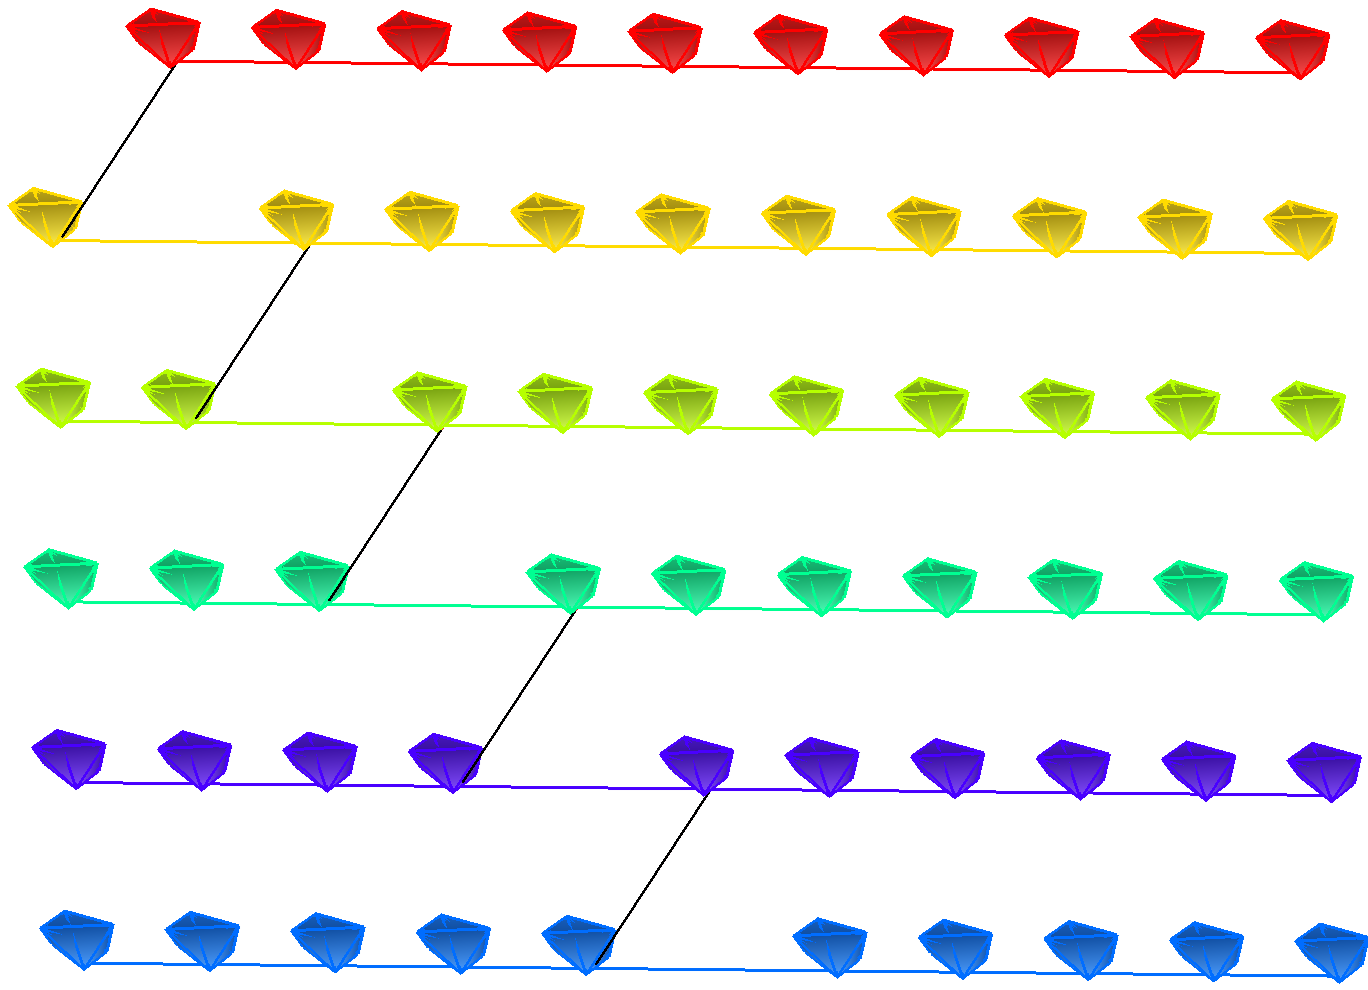
\includegraphics[width=.25\textwidth]{embedding.png}
	\hfill
	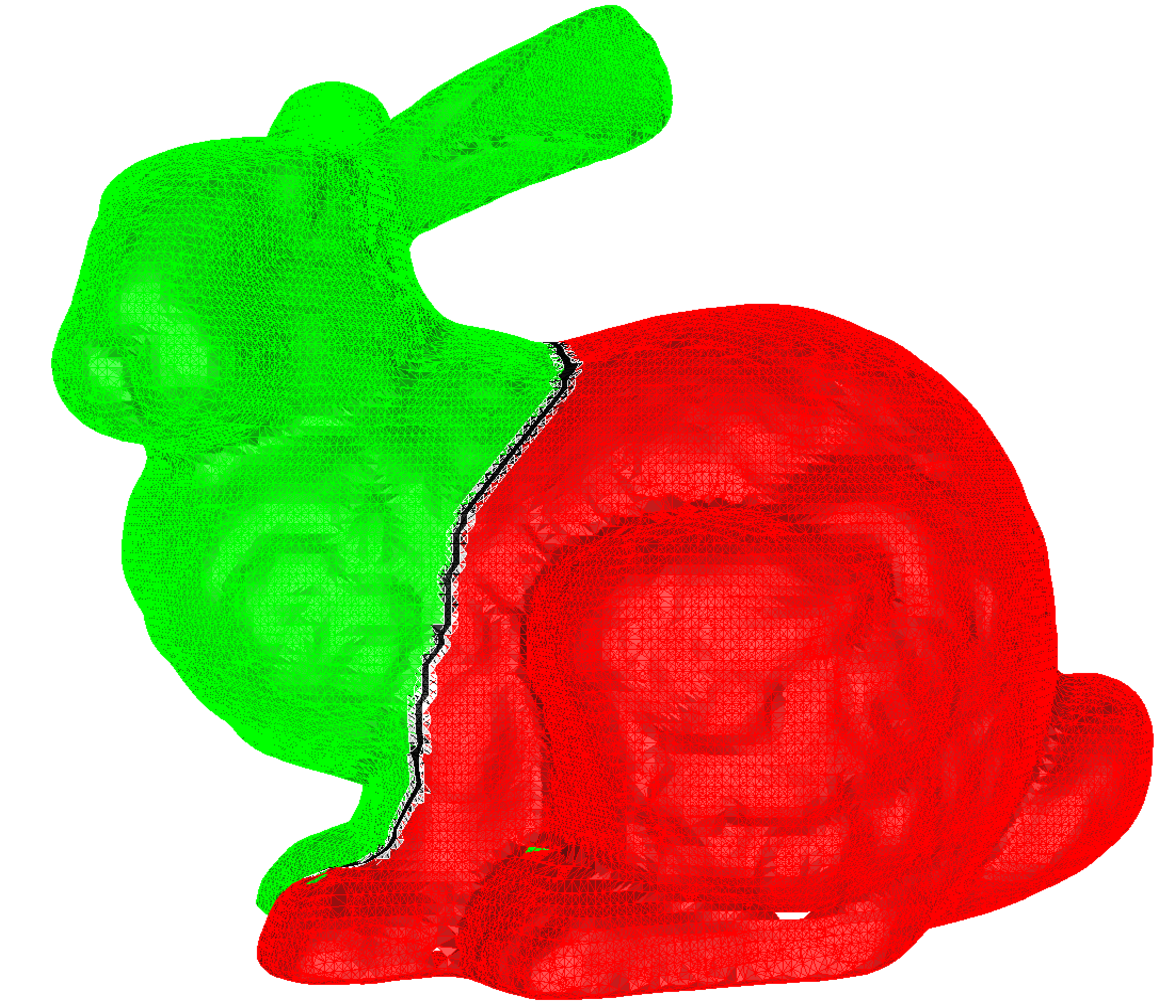
\includegraphics[width=.25\textwidth]{bunny-2.pdf}
	\hfill
	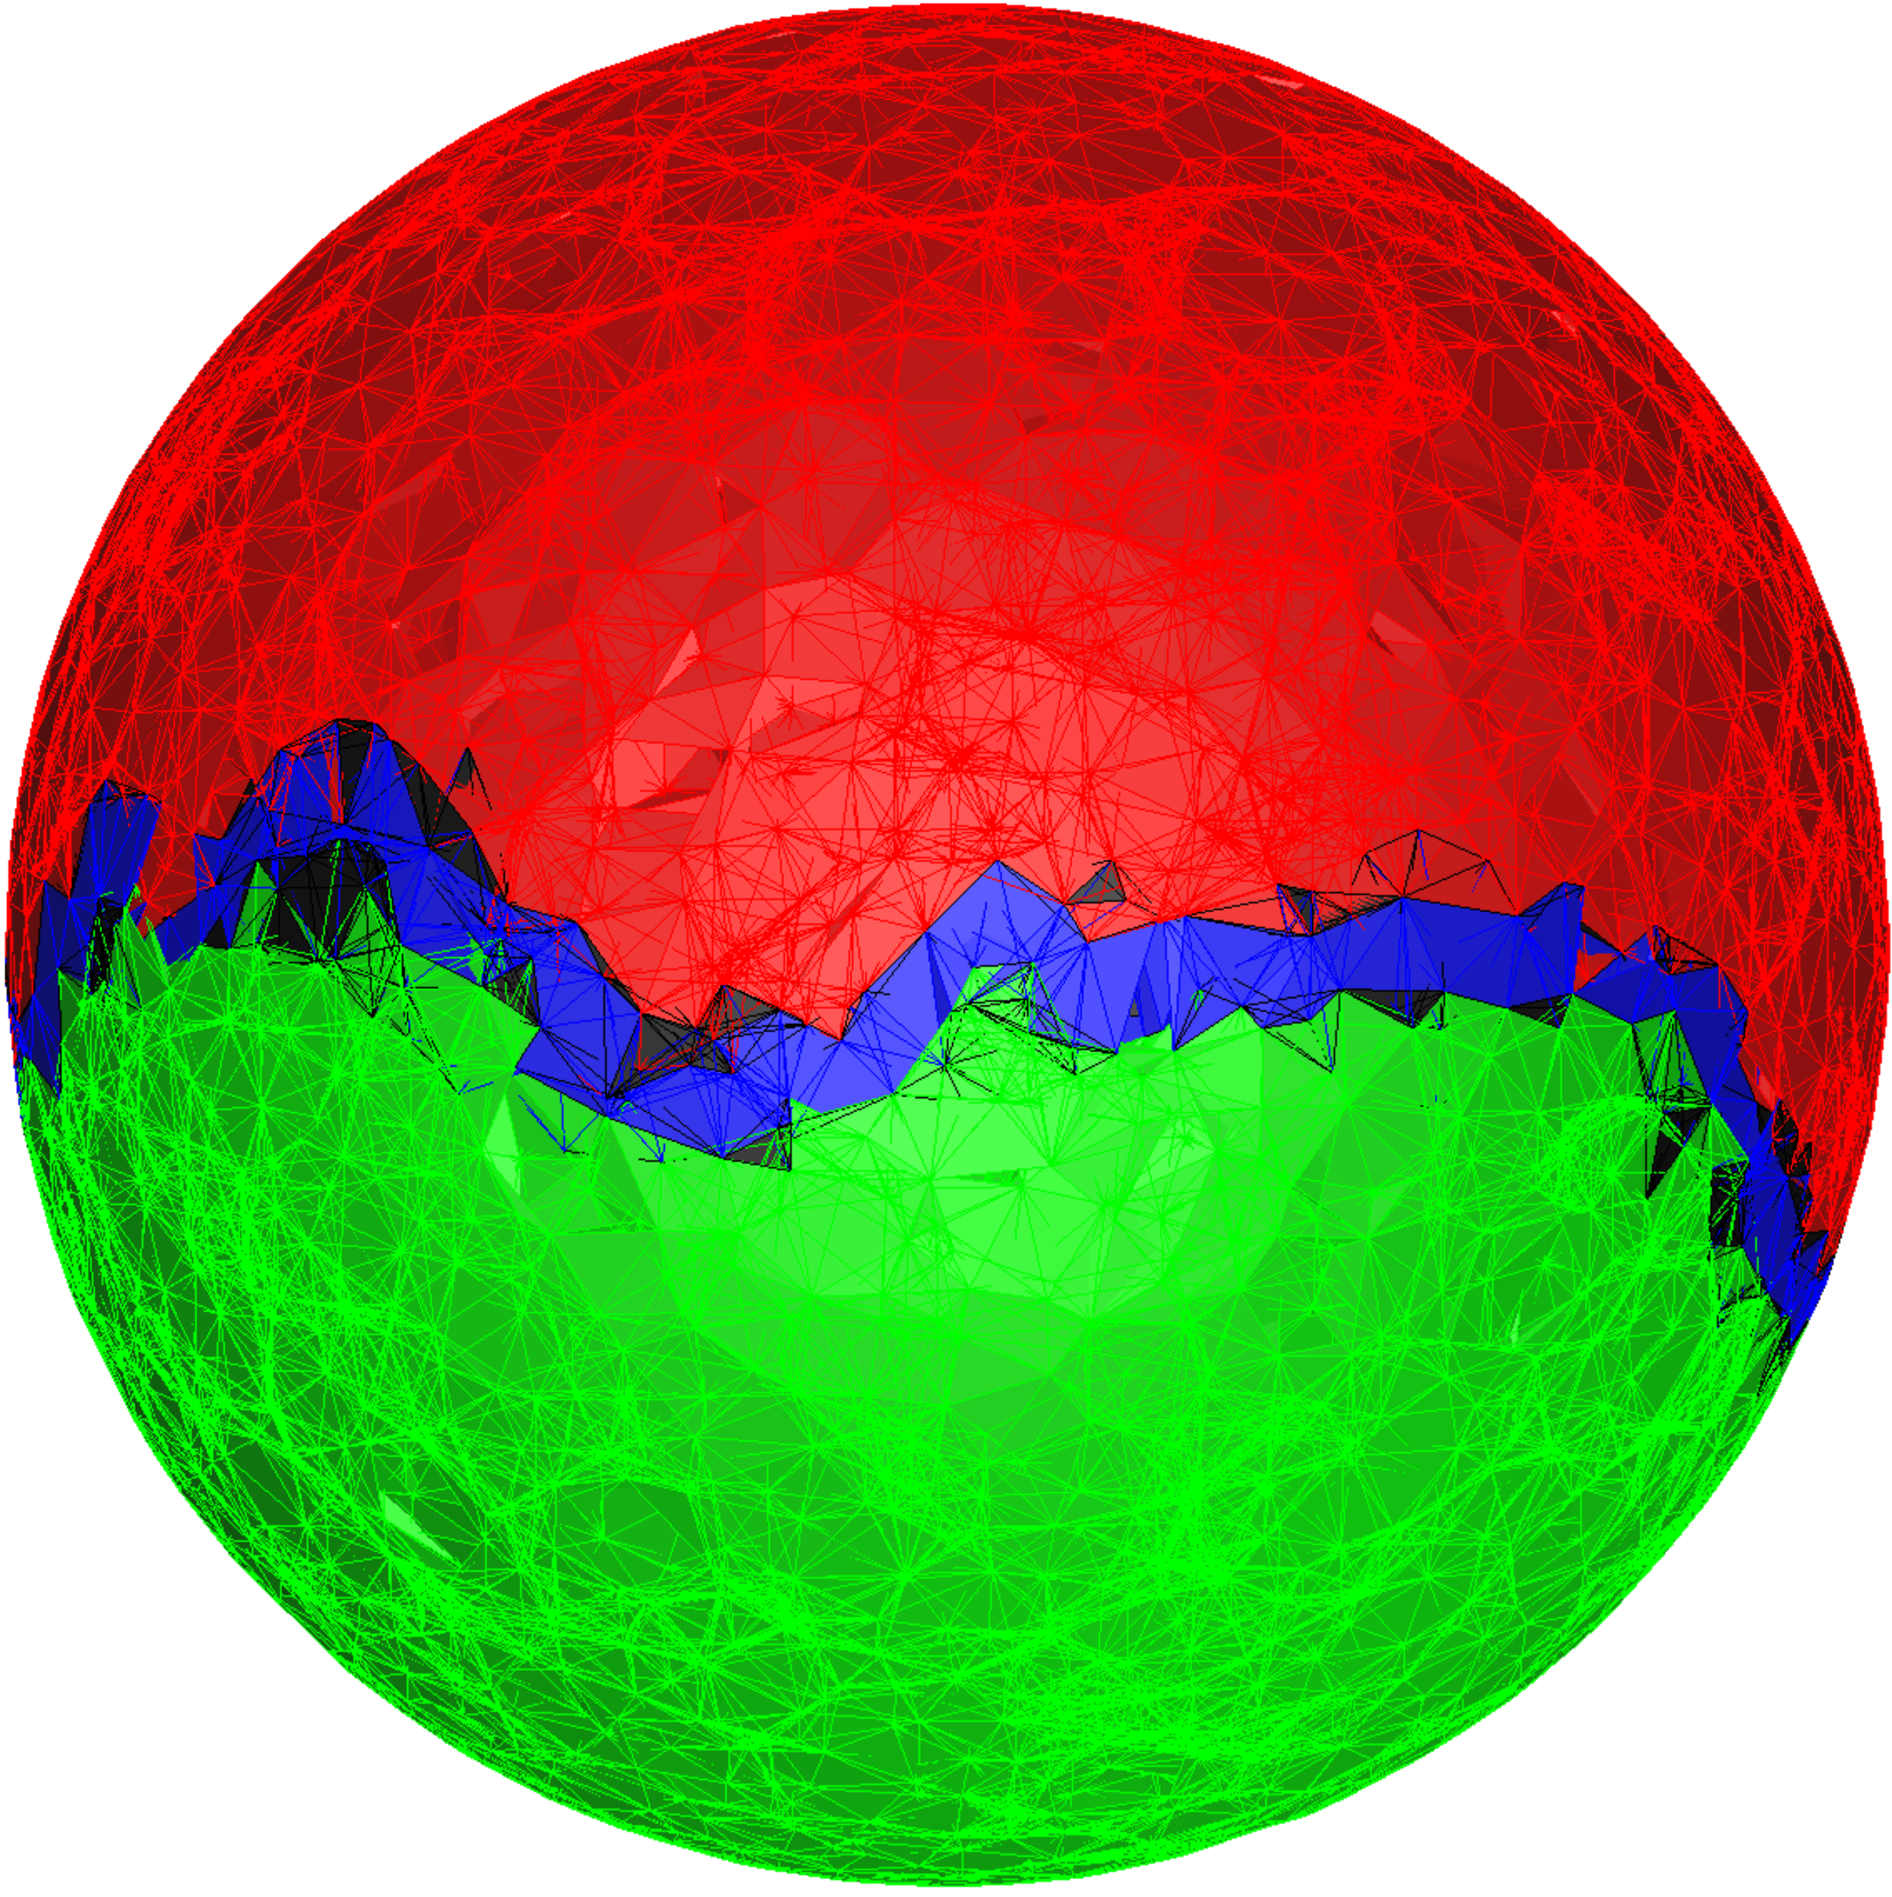
\includegraphics[width=.25\textwidth]{sphere-2.pdf}
\caption{Visualizations of {\multiblob}, {\bunny}, {\sphere}}
\end{figure}
\end{frame}

\begin{frame}
\begin{minipage}{.5\textwidth}
\centering
\begin{figure}
\centering
\begin{tikzpicture}[scale=.525]
\begin{axis}[xlabel=\# of partitions, ylabel={$\hat{\alpha}= \max_i \card{P_i} / \card{\K}$}, legend style={legend pos=north east, font=\small}]
\legend{\multiblob, \bunny, \clique, \gnp, \sphere, ideal}
\addplot table [x=num_partitions, y=graph_balance_ratio, col sep=comma] {pgf-speedup-figs/results/concurrent_homology/clique.11.22720.csv};
\addplot table [x=num_partitions, y=graph_balance_ratio, col sep=comma] {pgf-speedup-figs/results/concurrent_homology/bunny..05.csv};
\addplot table [x=num_partitions, y=graph_balance_ratio, col sep=comma] {pgf-speedup-figs/results/concurrent_homology/clique.20.csv};
\addplot table [x=num_partitions, y=graph_balance_ratio, col sep=comma] {pgf-speedup-figs/results/concurrent_homology/gnp.1250.047.csv};
\addplot table [x=num_partitions, y=graph_balance_ratio, col sep=comma] {pgf-speedup-figs/results/concurrent_homology/sphere.csv};
\addplot[dash pattern=on 4pt off 1pt on 4pt off 4pt, domain=2:10]{1/x};
\end{axis}
\end{tikzpicture}
\caption{Partition Balance Ratio $\hat{\alpha}$}
\end{figure}
\end{minipage}
\begin{minipage}{.5\textwidth}
\begin{figure}
\centering
\begin{tikzpicture}[scale=.525]
%\pgfplotsset{ymax=5}
\begin{axis}[xlabel=\# of partitions, ymax=50000, ylabel={\# of edges}, legend style={legend pos=north west, font=\small}]
\legend{\multiblob, \bunny, \clique, \gnp, \sphere, ideal}
\addplot table [x=num_partitions, skip coords between index={0}{1}, y=edgecut, col sep=comma, ignore chars=']
{pgf-speedup-figs/results/concurrent_homology/clique.11.22720.csv};
\addplot table [x=num_partitions, skip coords between index={0}{1}, y=edgecut, col sep=comma, ignore chars=']
{pgf-speedup-figs/results/concurrent_homology/bunny..05.csv};
\addplot table [x=num_partitions, skip coords between index={0}{1}, y=edgecut, col sep=comma, ignore chars=']
{pgf-speedup-figs/results/concurrent_homology/clique.20.csv};
\addplot table [x=num_partitions, skip coords between index={0}{1}, y=edgecut, col sep=comma, ignore chars=']
{pgf-speedup-figs/results/concurrent_homology/gnp.1250.047.csv};
\addplot table [x=num_partitions, skip coords between index={0}{1}, y=edgecut, col sep=comma, ignore chars=']
{pgf-speedup-figs/results/concurrent_homology/sphere.csv};
\end{axis}
\end{tikzpicture}
\caption{Edgecut}
\end{figure}
\end{minipage}
\begin{minipage}{.5\textwidth}
\centering
\begin{figure}
\begin{tikzpicture}[scale=.525]
\begin{axis}[xlabel=\# of partitions, ylabel={$\alpha = \max_i \card{\C_i} / \card{\K}$}, legend style={legend pos=north east, font=\small},legend style={at={(.95,.55)},anchor=east}]
\legend{\multiblob, \bunny, \clique, \gnp, \sphere, ideal}
\addplot table [x=num_partitions, y=cover_balance_ratio, col sep=comma,skip coords between index={0}{1}] 
{pgf-speedup-figs/results/concurrent_homology/clique.11.22720.csv};
\addplot table [x=num_partitions, y=cover_balance_ratio, col sep=comma, skip coords between index={0}{1}] 
{pgf-speedup-figs/results/concurrent_homology/bunny..05.csv};
\addplot table [x=num_partitions,skip coords between index={0}{1}, y=cover_balance_ratio, col sep=comma] 
{pgf-speedup-figs/results/concurrent_homology/clique.20.csv};
\addplot table [x=num_partitions, skip coords between index={0}{1},y=cover_balance_ratio, col sep=comma] 
{pgf-speedup-figs/results/concurrent_homology/gnp.1250.047.csv};
\addplot table [x=num_partitions, skip coords between index={0}{1},y=cover_balance_ratio, col sep=comma] 
{pgf-speedup-figs/results/concurrent_homology/sphere.csv};
\addplot[dash pattern=on 4pt off 1pt on 4pt off 4pt, domain=2:10]{1/x};
\end{axis}
\end{tikzpicture}
\caption{Balance Ratio for $\C$}
\end{figure}
\end{minipage}
\begin{minipage}{.5\textwidth}
\begin{figure}
\centering
\begin{tikzpicture}[scale=.525]
\begin{axis}[xlabel=\# of partitions, ylabel=$\ratio$, legend style={legend pos=north east, font=\small},legend style={at={(.95,.55)},anchor=east}]
\legend{\multiblob, \bunny, \clique, \gnp, \sphere, worst case}
\addplot table [x=num_partitions, y=blowup_factor, col sep=comma,skip coords between index={0}{1}] 
{pgf-speedup-figs/results/concurrent_homology/clique.11.22720.csv};
\addplot table [x=num_partitions, y=blowup_factor, col sep=comma, skip coords between index={0}{1}] 
{pgf-speedup-figs/results/concurrent_homology/bunny..05.csv};
\addplot table [x=num_partitions,skip coords between index={0}{1}, y=blowup_factor, col sep=comma] 
{pgf-speedup-figs/results/concurrent_homology/clique.20.csv};
\addplot table [x=num_partitions, skip coords between index={0}{1},y=blowup_factor, col sep=comma] 
{pgf-speedup-figs/results/concurrent_homology/gnp.1250.047.csv};
\addplot table [x=num_partitions, skip coords between index={0}{1},y=blowup_factor, col sep=comma] 
{pgf-speedup-figs/results/concurrent_homology/sphere.csv};
\addplot[dash pattern=on 4pt off 1pt on 4pt off 4pt, domain=2:10]{3};
\end{axis}
\end{tikzpicture}
\caption{Blowup Factor}
\label{fig:blowup-factors}
\end{figure}
\end{minipage}
\end{frame}

\begin{frame}
\begin{figure}
\centering
\begin{tikzpicture}[scale=.55]
\begin{semilogyaxis}[
name=plot1,
ymin=.09,
ymax=25,
xmin=0,
xmax=12,
xlabel=\# of  threads, 
title={$Multicore-Homology$},
ylabel= time to reduce boundary matrix (seconds),
minor y tick num={5},
legend style={at = {(.25,.6)}, font=\large}]
%\legend{\multiblob, \bunny, \clique, \gnp, \sphere}
\addplot table [x=num_threads, y=persistence, col sep=comma] {pgf-speedup-figs/results/concurrent_homology/clique.11.22720.csv};
\addplot table [x=num_threads, y=persistence, col sep=comma] {pgf-speedup-figs/results/concurrent_homology/bunny..05.csv};
\addplot table [x=num_threads, y=persistence, col sep=comma] {pgf-speedup-figs/results/concurrent_homology/clique.20.csv};
\addplot table [x=num_threads, y=persistence, col sep=comma] {pgf-speedup-figs/results/concurrent_homology/gnp.1250.047.csv};
\addplot table [x=num_threads, y=persistence, col sep=comma] {pgf-speedup-figs/results/concurrent_homology/sphere.csv};
\end{semilogyaxis}
\begin{semilogyaxis}[
name=plot3,
at=(plot1.below south east), anchor=above north east,
ymin=.09,
ymax=25,
xmin=0,
xmax=12,
xlabel= \# of threads,
title={$Heuristic-MH$},
%ylabel= time to reduce boundary matrix (seconds),
minor y tick num={5},
legend style={at={(1,.55)}, font=\large}]
%\legend{\multiblob, \bunny, \clique, \gnp, \sphere}
\addplot table [x=num_partitions, y=persistence, col sep=comma] {pgf-speedup-figs/results/cover_homology/clique.11.22720.csv};
\addplot table [x=num_partitions, y=persistence, col sep=comma] {pgf-speedup-figs/results/cover_homology/bunny..05.csv};
\addplot table [x=num_partitions, y=persistence, col sep=comma] {pgf-speedup-figs/results/cover_homology/clique.20.csv};
\addplot table [x=num_partitions, y=persistence, col sep=comma] {pgf-speedup-figs/results/cover_homology/gnp.1250.047.csv};
\addplot table [x=num_partitions, y=persistence, col sep=comma] {pgf-speedup-figs/results/cover_homology/sphere.csv};
\end{semilogyaxis}

\begin{semilogyaxis}[
name=plot4,
at=(plot3.right of north east), anchor=left of north west,
ymin=.09,
ymax=25,
xmin=0,
xmax=12,
xlabel= \# of threads, 
title={$Spectral-Sequence$},
minor y tick num={5},
legend style={at={(.95,.525)}, font=\large}]
\legend{\multiblob, \bunny, \clique, \gnp, \sphere}
\addplot table [x=num_partitions, y=persistence, col sep=comma] {pgf-speedup-figs/results/phat_14_ss/clique.11.22720.csv};
\addplot table [x=num_partitions, y=persistence, col sep=comma] {pgf-speedup-figs/results/phat_14_ss/bunny..05.csv};
\addplot table [x=num_partitions, y=persistence, col sep=comma] {pgf-speedup-figs/results/phat_14_ss/clique.20.csv};
\addplot table [x=num_partitions, y=persistence, col sep=comma] {pgf-speedup-figs/results/phat_14_ss/gnp.1250.047.csv};
\addplot table [x=num_partitions,, y=persistence, col sep=comma] {pgf-speedup-figs/results/phat_14_ss/sphere.csv};
\end{semilogyaxis}

\begin{semilogyaxis}[
name=plot2,
at=(plot4.above north west),
anchor = below south west,
ymin=.09,
ymax=25,
xmin=0,
xmax=12,
xlabel=\# of  threads,
title={$Chunk$},
minor y tick num={5},
legend style={at={(.95,.525)}, font=\large}]
%\legend{\multiblob, \bunny, \clique, \gnp, \sphere}
\addplot table [x=num_partitions, y=persistence, col sep=comma] {pgf-speedup-figs/results/phat_14_chunk/clique.11.22720.csv};
\addplot table [x=num_partitions, y=persistence, col sep=comma] {pgf-speedup-figs/results/phat_14_chunk/bunny..05.csv};
\addplot table [x=num_partitions, y=persistence, col sep=comma] {pgf-speedup-figs/results/phat_14_chunk/clique.20.csv};
\addplot table [x=num_partitions, y=persistence, col sep=comma] {pgf-speedup-figs/results/phat_14_chunk/gnp.1250.047.csv};
\addplot table [x=num_partitions,, y=persistence, col sep=comma] {pgf-speedup-figs/results/phat_14_chunk/sphere.csv};
\end{semilogyaxis}
\end{tikzpicture}
\caption{Time to reduce the boundary matrix for each algorithm.}
\label{fig:ctl_vs_phat}
\end{figure}

\end{frame}
